\documentclass[xelatex,12pt]{beamer}
\usepackage{pgfpages}
\usepackage{fontspec}
\usepackage{xunicode}
\usepackage{polyglossia}
\PolyglossiaSetup{french}{indentfirst=false}
\usepackage[french=guillemets]{csquotes}
\usepackage{xpatch}
\usepackage{diagbox}

\setmainlanguage{french}
\xapptocmd\ttfamily{\XeTeXinterchartokenstate=0 }{}{}
\newcommand{\nospace}[1]{\texttt{#1}}

\usepackage{algorithm}
\usepackage[noend]{algpseudocode}
    \newcounter{lastenum}
    \newcommand{\mtpause}{\setcounter{lastenum}{\value{enumi}}}
    \newcommand{\mtresume}{\setcounter{enumi}{\value{lastenum}}}
\resetcounteronoverlays{lastenum}

\usepackage[backend=biber, style=chem-acs]{biblatex}
\addbibresource{diapo.bib} 
\setbeamertemplate{bibliography item}[triangle]

\usepackage[labelformat=empty]{caption}
\usepackage{graphicx}

\usepackage{multirow}% row fusion
\usepackage{array} % column fusion
\usepackage{xfrac} % small fractions
\usepackage{adjustbox}
\usepackage{listings}

\usepackage{color}
\definecolor{gray}{rgb}{0.4,0.4,0.4}
\definecolor{white}{rgb}{1, 1, 1}
\definecolor{darkblue}{rgb}{0.0,0.0,0.6}
\definecolor{cyan}{rgb}{0.0,0.6,0.6}
\definecolor{blue}{rgb}{0, .505, .949}

\usetheme{Warsaw}

\setbeamertemplate{frametitle}{\nointerlineskip  
    \begin{beamercolorbox}[wd=\paperwidth,ht=2.75ex,dp=1.375ex]{frametitle}
        \hspace*{2ex}\insertframetitle \hfill {\small\insertframenumber/\inserttotalframenumber} \hspace*{1ex}%
    \end{beamercolorbox}}
\setbeamercolor{beamercolorbox}{fg=blue}
\setbeamercolor*{palette tertiary}{bg=blue}
\setbeamercolor{frametitle}{fg=white, bg=black}
\setbeamercolor{palette primary}{fg=black, bg=white}
\setbeamercolor{title}{fg=white, bg=black}

\usepackage{color}

\setbeameroption{hide notes} % Only slides
%\setbeameroption{show only notes} % Only notes
%\setbeameroption{show notes on second screen=right} % Both

\setbeamertemplate{itemize items}[ball]
\setbeamercolor{itemize items}{fg=darkblue}

 \titlegraphic{\vspace{-1cm}
      
\includegraphics[width=2.5cm]{images/paris8_1}\hspace*{4.75cm}~%
      \hfill
      
\includegraphics[width=2.5cm]{images/logo}
}

 
\title{Projet dirigé}
\subtitle{Réseaux de neurones liés au moteur de recherche}
\author[\textsc{P. Gajenthran}]{\textsc{Panchalingamoorthy Gajenthran}}
\institute{\normalsize Université Paris 8, LIASD}
 

\beamertemplatenavigationsymbolsempty
\setbeamertemplate{blocks}[rounded][shadow=false]
\setbeamerfont{page number in head/foot}{size=\large}

\setbeamertemplate{itemize item}{\color{black}$\bullet$}

\begin{document}
{ \setbeamertemplate{headline}{}
  \setbeamertemplate{footline}{}
  \begin{frame}
  \titlepage
  \end{frame}

}

\section{Introduction}

\begin{frame}{Introduction}
Ceci est l'introduction.
\end{frame}

\section{Développement} 
\subsection{Sous Développement 1}
\begin{frame}{SS1}
  \begin{figure}[ht]
    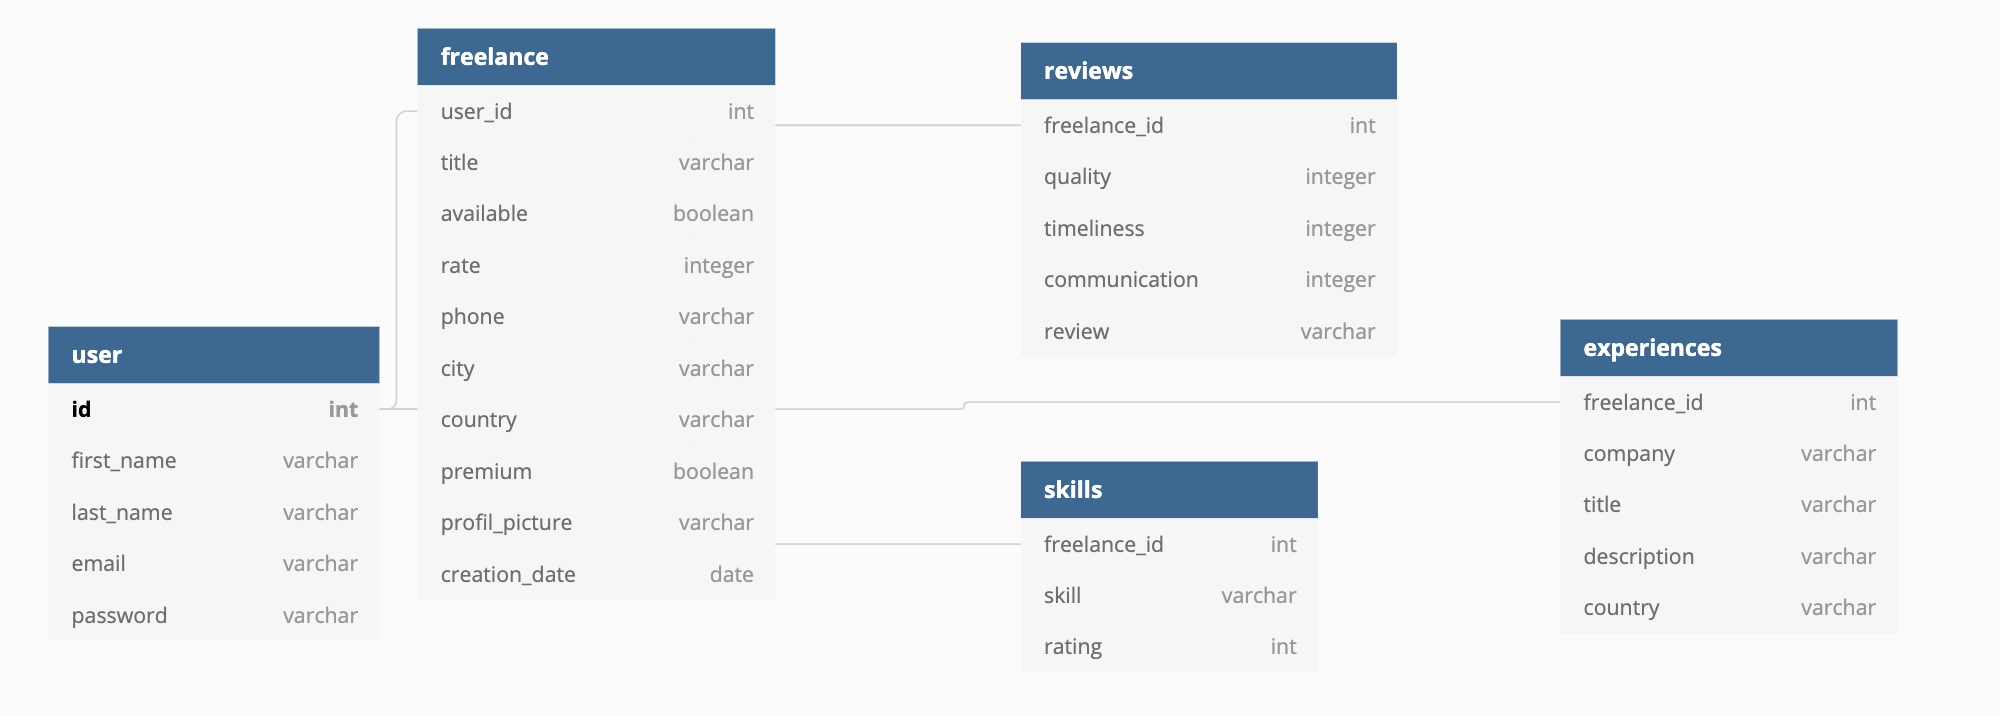
\includegraphics[scale=0.33]{images/diagram}
    \caption{Diagramme représentant la base de données des freelances}
  \end{figure}
\end{frame}

\subsection{Sous Développement 2}
\begin{frame}{SS2}
  \begin{itemize}
    \item Texte en \textit{italique}
    \item Texte en \texttt{gras}
  \end{itemize}
\end{frame}

\section{Conclusion}
\begin{frame}{Conclusion}
\end{frame}

\begin{frame}{Références}
  \begin{itemize}
    \item Ansh Balde (2019). Search Engines and Neural Networks
    \item Yang Li, Ting Liu (2016). Hashtag Recommendation with Topical Attention-Based LSTM
    \item Nikhil Dandekar (2016). What are some uses of machine learning in search engines?
    \item Rauber, A., D. Merkl, et M. Dittenbach (2002). The growing hierarchical self-organizing map:exploratory analysis of high-dimensional data. \textit{IEEE Transactions on Neural Networks 13},1331–1341
  \end{itemize}
\end{frame}

\end{document}
